
\section{Object representation}
\begin{frame}{Object representation}
\begin{itemize}
    \item Volumetric
    \item Surface
    \begin{itemize}
        \item Triangulated mesh
        \item Nurbs
    \end{itemize}
\end{itemize}

\end{frame}

\begin{frame}[t,allowframebreaks]{3D Vision}
    \tableofcontents
    
\end{frame}

\begin{frame}{Object representation}
\begin{itemize}
    \item Geometry
    \item Topology
\end{itemize}
\end{frame}

\subsection{Geometry and Topology}
\begin{frame}{Geometry and Topology}
    \begin{columns}
        \column{0.6\textwidth}
            \begin{block}{Geometry}
            Geometry 
            % (from the Ancient Greek: γεωμετρία; geo- "earth", -metron "measurement") 
            is a branch of mathematics concerned with questions of shape, size, relative position of figures, and the properties of space \cite{de2015mathematizing}. A mathematician who works in the field of geometry is called a geometer.
            \end{block}
            \begin{block}{Topology}
            In mathematics, topology 
            % (from the Greek τόπος, 'place', and λόγος, 'study')
            is concerned with the properties of a geometric object that are preserved under continuous deformations, such as stretching, twisting, crumpling and bending, but not tearing or gluing.
            \end{block}
        \column{0.4\textwidth}
            \begin{figure}
                \centering
                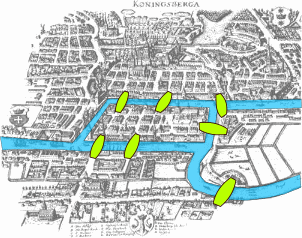
\includegraphics[width=\textwidth]{figs/Konigsberg_bridges.png}
                \caption{Seven Bridges of Königsberg 
                    \cite{euler1953leonhard, euler1741solutio,wiki:7bridges}
                }
            \end{figure}
    \end{columns}
    
    
\end{frame}


\begin{frame}[fragile]{OBJ file format}
    \begin{columns}
        \column{0.6\textwidth}
        Content of \verb+example.obj+ can be displayed with ParaView application.
            \begin{lstlisting}
            v 0.0 0.0 0.1
            v 0.0 0.1 1.0
            v 0.0 1.0 0.1
            v 0.0 1.0 1.0
            v 0.2 2.0 0.5
            
            g cellobject
            f 1 2 4 3
            f 3 4 5
            \end{lstlisting}
        \column{0.4\textwidth}
            \begin{figure}
                \centering
                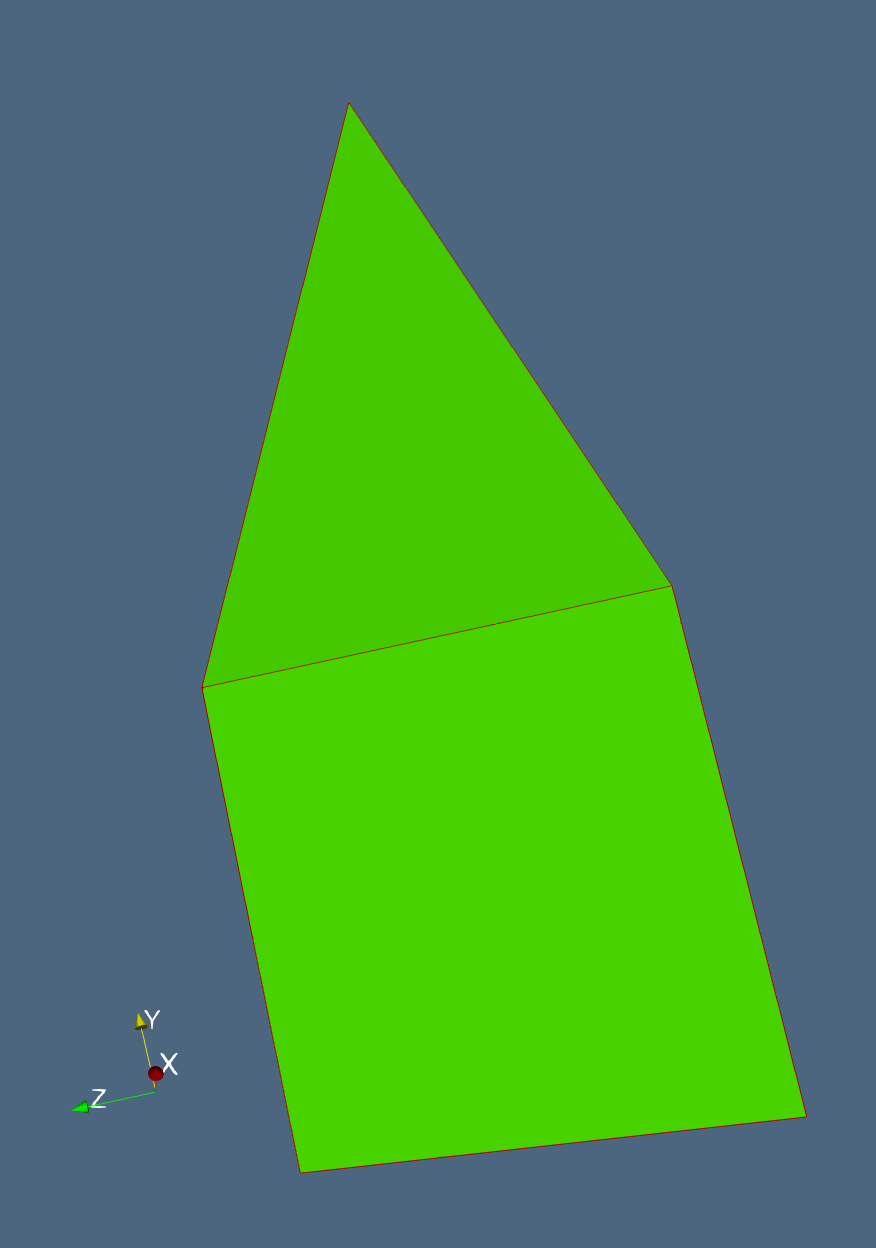
\includegraphics[width=\textwidth]{figs/example_obj.png}
                % \caption{Caption}
                % \label{fig:my_label}
            \end{figure}
    \end{columns}
\end{frame}

\begin{frame}{Linear Algebraic Representation\cite{DiCarlo2014}}
    
\end{frame}

\begin{frame}
\begin{figure}
    \centering
    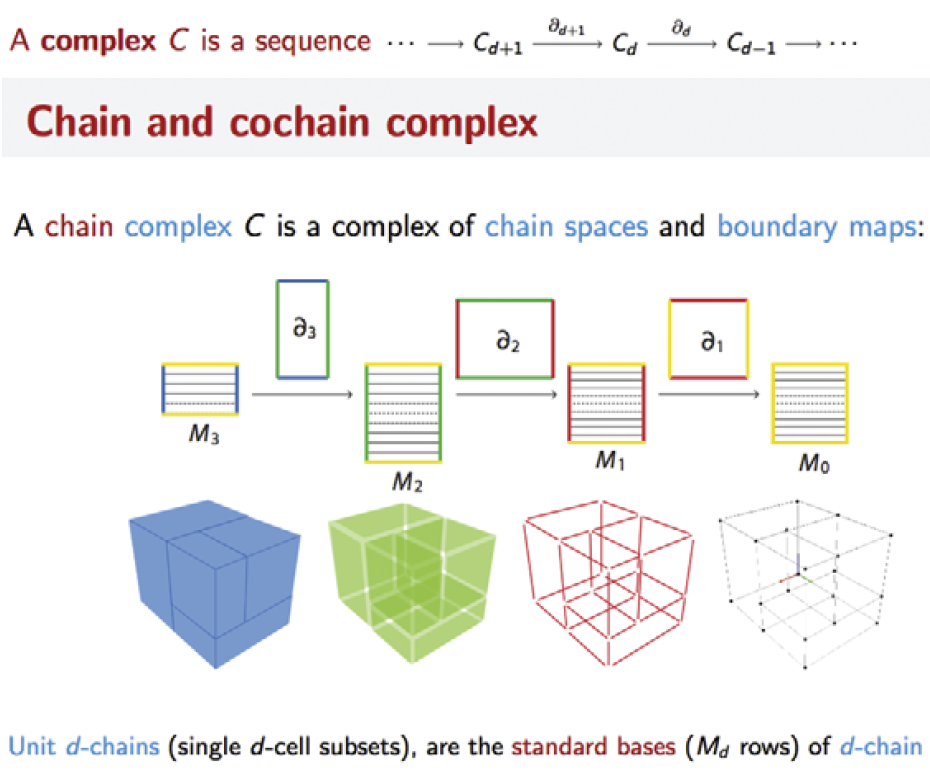
\includegraphics[width=\textwidth]{figs/L02-chain-complex.png}
    % \caption{Caption}
    % \label{fig:my_label}
\end{figure}
    
\end{frame}

\begin{frame}
\begin{figure}
    \centering
    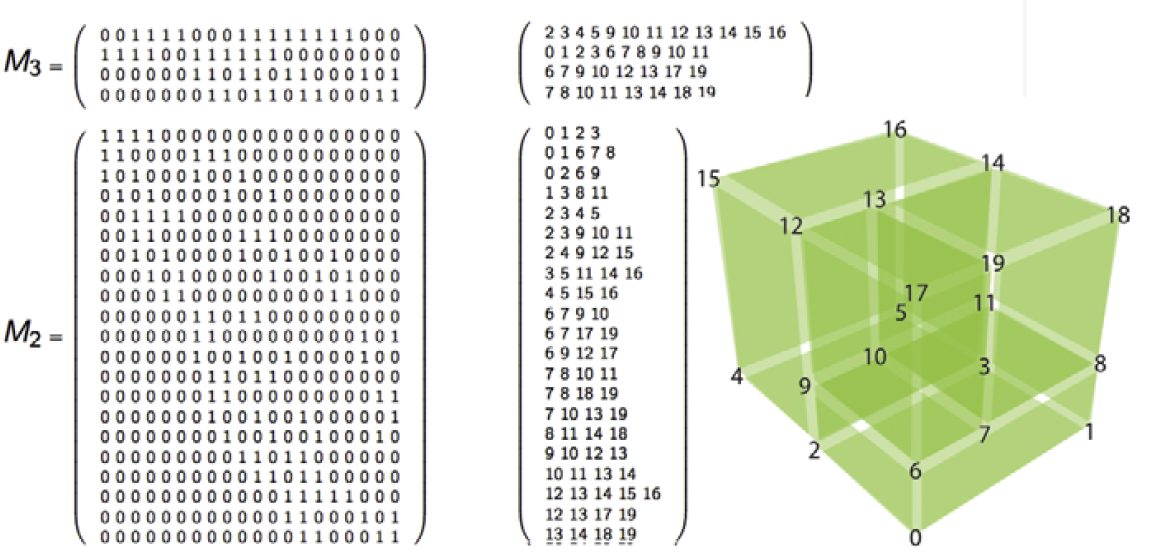
\includegraphics[width=\textwidth]{figs/L02-characteristic-matrices.png}
    % \caption{Caption}
    % \label{fig:my_label}
\end{figure}
    
\end{frame}


\subsection{Delaunay triangulation}
\begin{frame}{Triangulation (terrain map)}
\begin{figure}
    \centering
    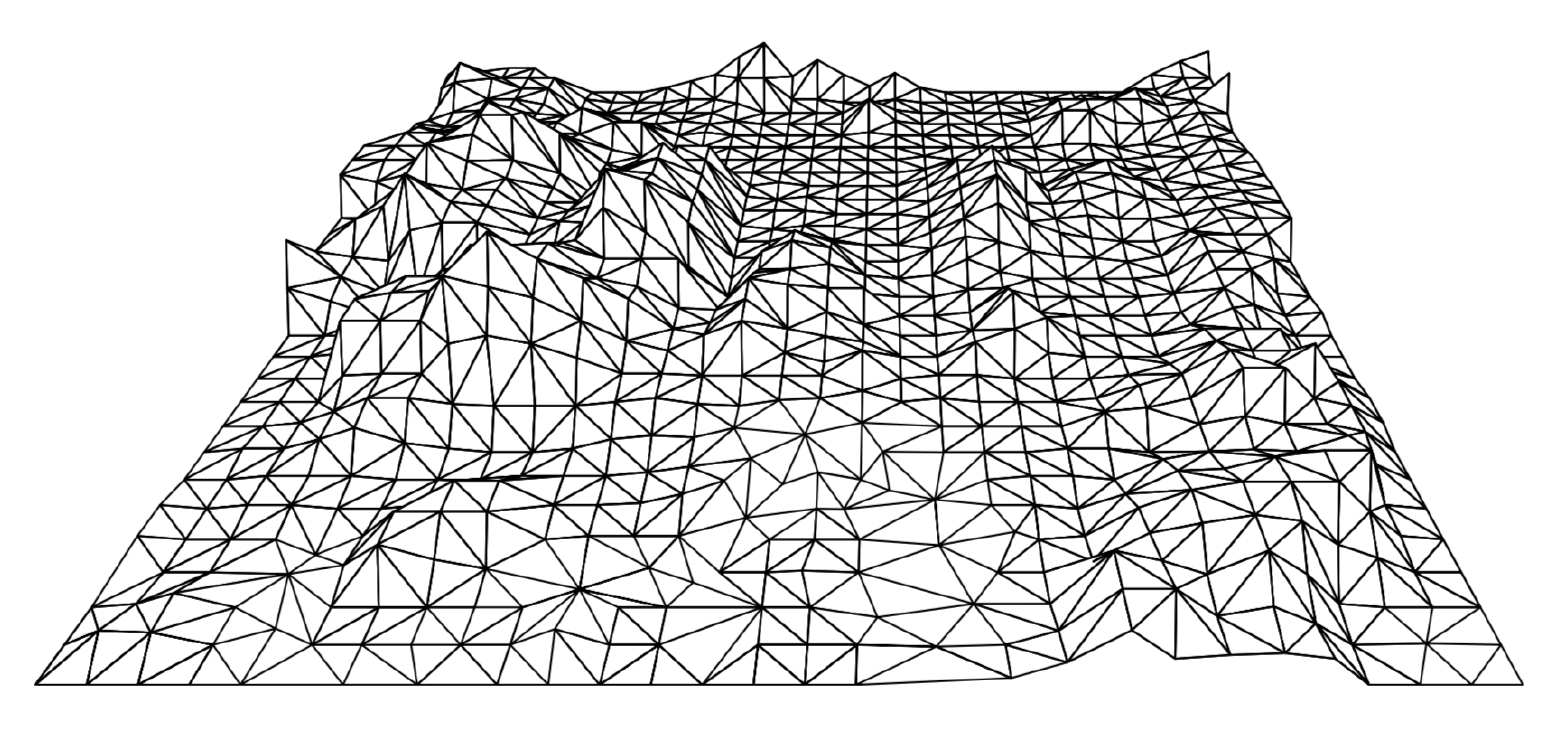
\includegraphics[width=\textwidth]{figs/L07-terrain-map.png}
    % \caption{Caption}
    % \label{fig:terrain-map}
\end{figure}

\end{frame}


\begin{frame}{Point cloud}
\begin{figure}
    \centering
    \includegraphics{}
    \caption{Caption}
    \label{fig:my_label}
\end{figure}
    
\end{frame}

\begin{frame}{Triangulation}

    \begin{columns}
    	\column{.6\textwidth}
    % 	\begin{block}{}
    We first determine a triangulation of P: a
    planar subdivision whose bounded faces are
    triangles and whose vertices are the points of
    P. We then lift each sample point to its height,
    mapping every triangle in the triangulation to
    a triangle in 3-space.
    
    We get is a polyhedral terrain, the graph of a
    piecewise linear continuous function
    The polyhedral terrain as an approximation of
    the original terrain.    
    % 	\end{block}
    	\column{.4\textwidth}
    % 	\begin{block}{Generative}
    	\begin{figure}
    	    \centering
    	    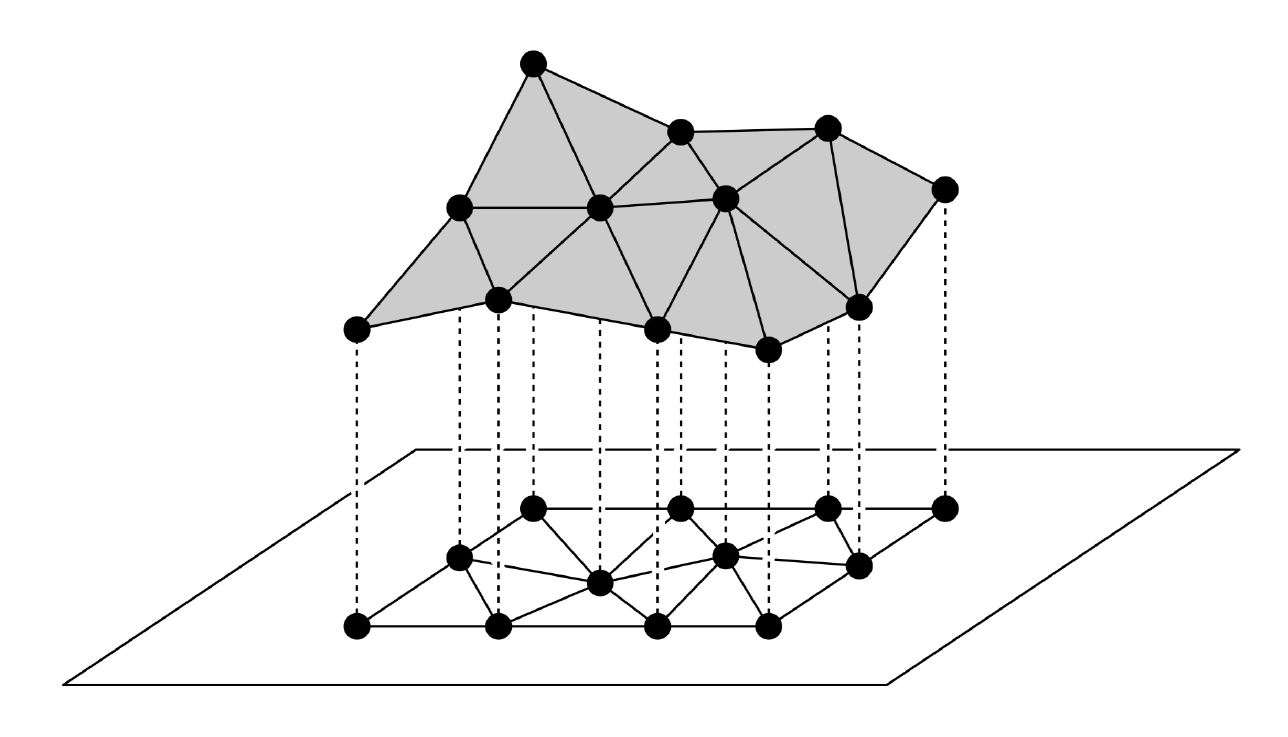
\includegraphics[width=\textwidth]{figs/L07-terrain-map-2.png}
    	   % \caption{Caption}
    	   % \label{fig:my_label}
    	\end{figure}
    % 	\end{block}
    \end{columns}

\end{frame}


\begin{frame}{Triangulations of Planar Point Sets \cite{DeBerg2008}}

    Let $P := \left\{p_1, p_2,..., p_n\right\}$ be a set of points in the plane. To be able to formally
    define a triangulation of P, we first define a maximal planar subdivision as
    a subdivision S such that no edge connecting two vertices can be added to
    S without destroying its planarity. In other words, any edge that is not in S
    intersects one of the existing edges. A triangulation of P is now defined as a
    maximal planar subdivision whose vertex set is P.
    \begin{columns}
        \column{0.6\textwidth}
     Let P be a set of n points in the plane, not all collinear, and let k
denote the number of points in P that lie on the boundary of the convex hull
of P. Then any triangulation of P has $2n - 2 - k$ triangles and $3n-3-k$ edges.
        \column{0.3\textwidth}
        \begin{figure}
            \centering
            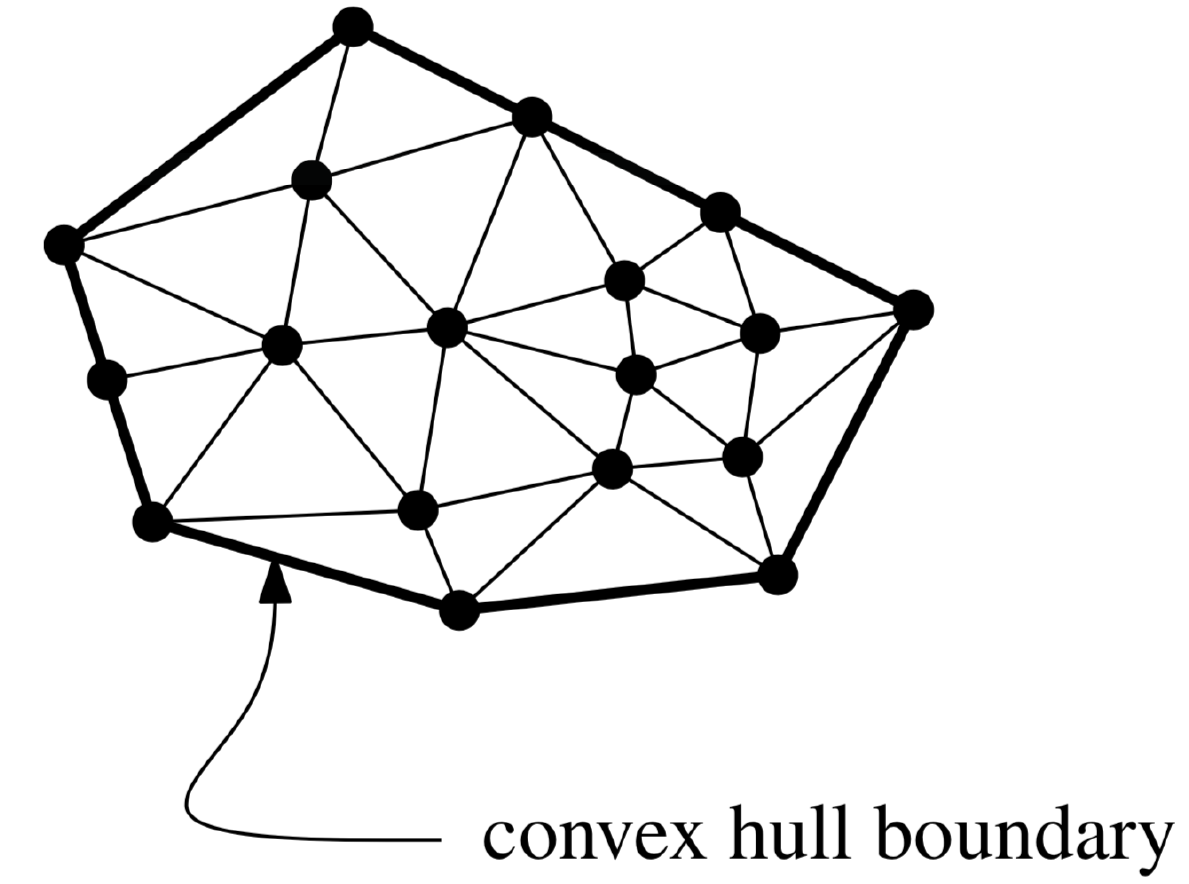
\includegraphics[width=\textwidth]{figs/L07-convex-hull.png}
            % \caption{Caption}
            % \label{fig:my_label}
        \end{figure}
    \end{columns}
\end{frame}


\begin{frame}{The Delaunay Triangulation}
    \begin{columns}
        \column{0.6\textwidth}
        Delaunay triangulation for a set P of discrete
points in a plane is a triangulation DT(P)
such that no point in P is inside the
circumcircle of any triangle in DT(P).

Delaunay triangulations maximize the
minimum angle of all the angles of the
triangles in the triangulation.
        \column{0.4\textwidth}
        \begin{figure}
            \centering
            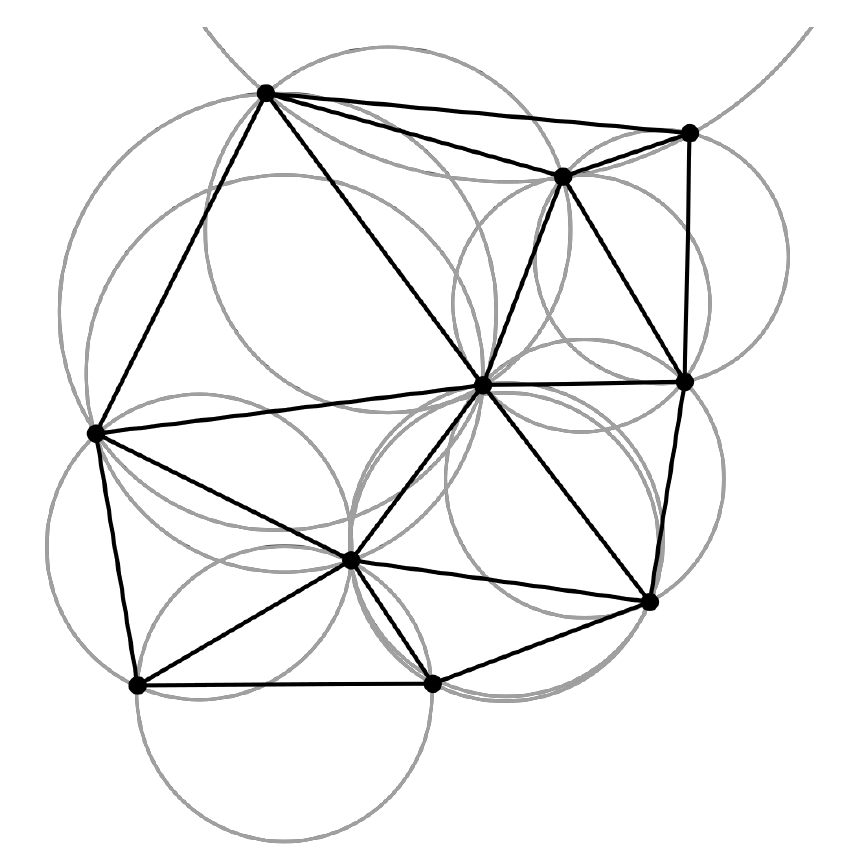
\includegraphics[width=\textwidth]{figs/L07-delaunay-triangulation.png}
            % \caption{Caption}
            % \label{fig:my_label}
        \end{figure}
    \end{columns}
\end{frame}

\begin{frame}{Delaunay Triangulation Properties}
\begin{itemize}
    \item The Delaunay triangulation is a triangulation which is equivalent to the
nerve of the cells in a Voronoi diagram,
    \item it is the triangulation of the convex hull of the points in the diagram in
which every circumcircle of a triangle is an empty circle
an edge is illegal if we can locally increase the smallest angle by flipping
that edge.
    \item A Delaunay triangulation is unique iff the circumcircle of every triangle
contains exactly three points on its circumference: the vertices of the
triangle.
    \item For instance, the Delaunay diagram of the four vertices of a square is a
square, and can be converted into a triangulation in two different ways
\end{itemize}
    
\end{frame}

\begin{frame}{Computing of The Delaunay Triangulation}
    \begin{columns}
        \column{0.7\textwidth}
        It turns out that it is not necessary to compute the angles to check whether a given edge is legal. Instead, we can use the simple criterion
stated in the next lemma. The correctness of this criterion follows from Thales's Theorem
\begin{block}{}
         Let edge $\overline{p_i p_j}$ be incident to triangles $p_i p_j p_k$ and $p_i p_j p_l$
, and let $C$ be the circle through $p_i$, $p_j$, and $p_k$. 
The edge $\overline{p_i p_j}$ is illegal if and only if the point $p_l$
lies in the interior of $C$. Furthermore, if the points $p_i$, $p_j$, $p_k$, $p_l$ form
a convex quadrilateral and do not lie on a common circle, then exactly one of
$\overline{p_i p_j}$ and $\overline{p_k p_l}$ is an illegal edge.
\end{block}
        \column{0.3\textwidth}
        \begin{figure}
            \centering
            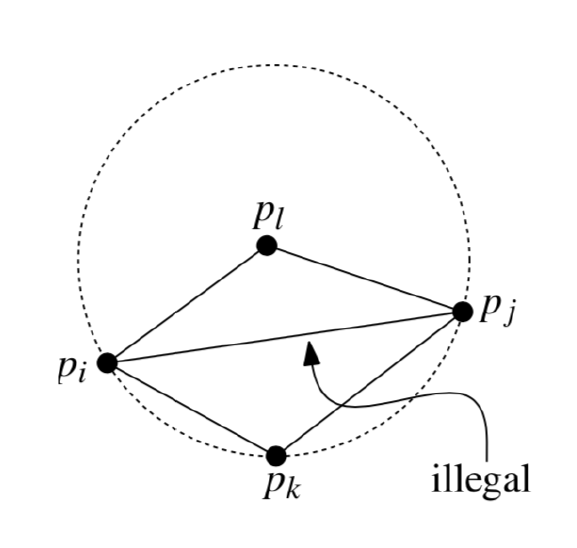
\includegraphics[width=\textwidth]{figs/L07-delaunay-triangulation-illegal.png}
            % \caption{Caption}
            % \label{fig:my_label}
        \end{figure}
    \end{columns}
\end{frame}

\begin{frame}{Computing the Delaunay Triangulation}

We define a legal triangulation to be a triangulation that does not contain
any illegal edge. From the observation above it follows that any angle-optimal
triangulation is legal. Computing a legal triangulation is quite simple, once we
are given an initial triangulation. We simply flip illegal edges until all edges are
legal.

\begin{algorithm}[H]
\SetAlgoLined
\KwIn{
Some triangulation T of a point set P.
}
\KwOut{
A legal triangulation of P.
}
 \While{T contains an illegal edge $\overline{p_i p_j}$}{
    % (Flip )\;
    \Begin(Flip $\overline{p_i p_j}$){
    Let $p_i p_j p_k$ and $p_i p_j p_l$ be the two triangles adjacent to $\overline{p_i p_j}$\;
    Remove $\overline{p_i p_j}$ from T, and add $\overline{p_k p_l}$ instead.
    }
 }
\Return {T}
%  \caption{How to write algorithms}
\end{algorithm}
\end{frame}

\begin{frame}{Voronoi complexes}
    
\end{frame}
\begin{frame}{Voronoi complexes}
    \begin{columns}
        \column{0.7\textwidth}
        \begin{itemize}
            \item  Voronoi diagram is a partitioning of a plane into regions based on distance
to points in a specific subset of the plane.
            \item
That set of points (called seeds, sites, or generators) is specified beforehand,
and for each seed there is a corresponding region consisting of all points
closer to that seed than to any other.  These regions are called Voronoi cells.
            \item
The Voronoi diagram of a set of points is dual to its Delaunay triangulation   
            
        \end{itemize}


        \column{0.3\textwidth}
        \begin{figure}
            \centering
            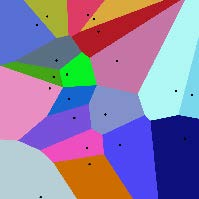
\includegraphics[width=\textwidth]{figs/L07-voronoi.jpg}
            % \caption{Caption}
            % \label{fig:my_label}
        \end{figure}
    \end{columns}
\end{frame}

    % \begin{columns}
    %     \column{0.6\textwidth}
    % \end{columns}
\begin{frame}{The post office problem}
    \begin{figure}
        \centering
        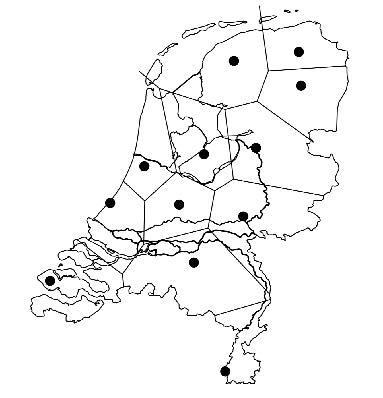
\includegraphics[width=0.5\textwidth]{figs/L07-post-office-problem.jpg}
        
        \caption{The post office problem \cite{DeBerg2008}}
        \label{fig:my_label}
    \end{figure}
    % \begin{columns}
    %     % \column{0.7\textwidth}
    %     % \column{0.3\textwidth}
    % \end{columns}
\end{frame}

% De Berg, M., Cheong, O., Van Kreveld, M., & Overmars, M. (2008). Computational geometry: Algorithms and applications. Computational Geometry: Algorithms and Applications. https://doi.org/10.1007/978-3-540-77974-2
\subsection{Convex hull}

\begin{frame}
\vfill
\centering

\begin{beamercolorbox}[sep=8pt,center,shadow=true,rounded=true]{title}
Convex Hull
\end{beamercolorbox}
\vfill
    
\end{frame}




\begin{frame}{Convex Hull}
    \begin{columns}
        \column{0.6\textwidth}
            Given a discrete set S of points:
            \begin{itemize}
                \item intersection of all convex sets containing S;
                \item minimum convex set containing S
                \item set spanned by all convex combinations of S points
            \end{itemize}
        \column{0.4\textwidth}
        \begin{figure}
            \centering
            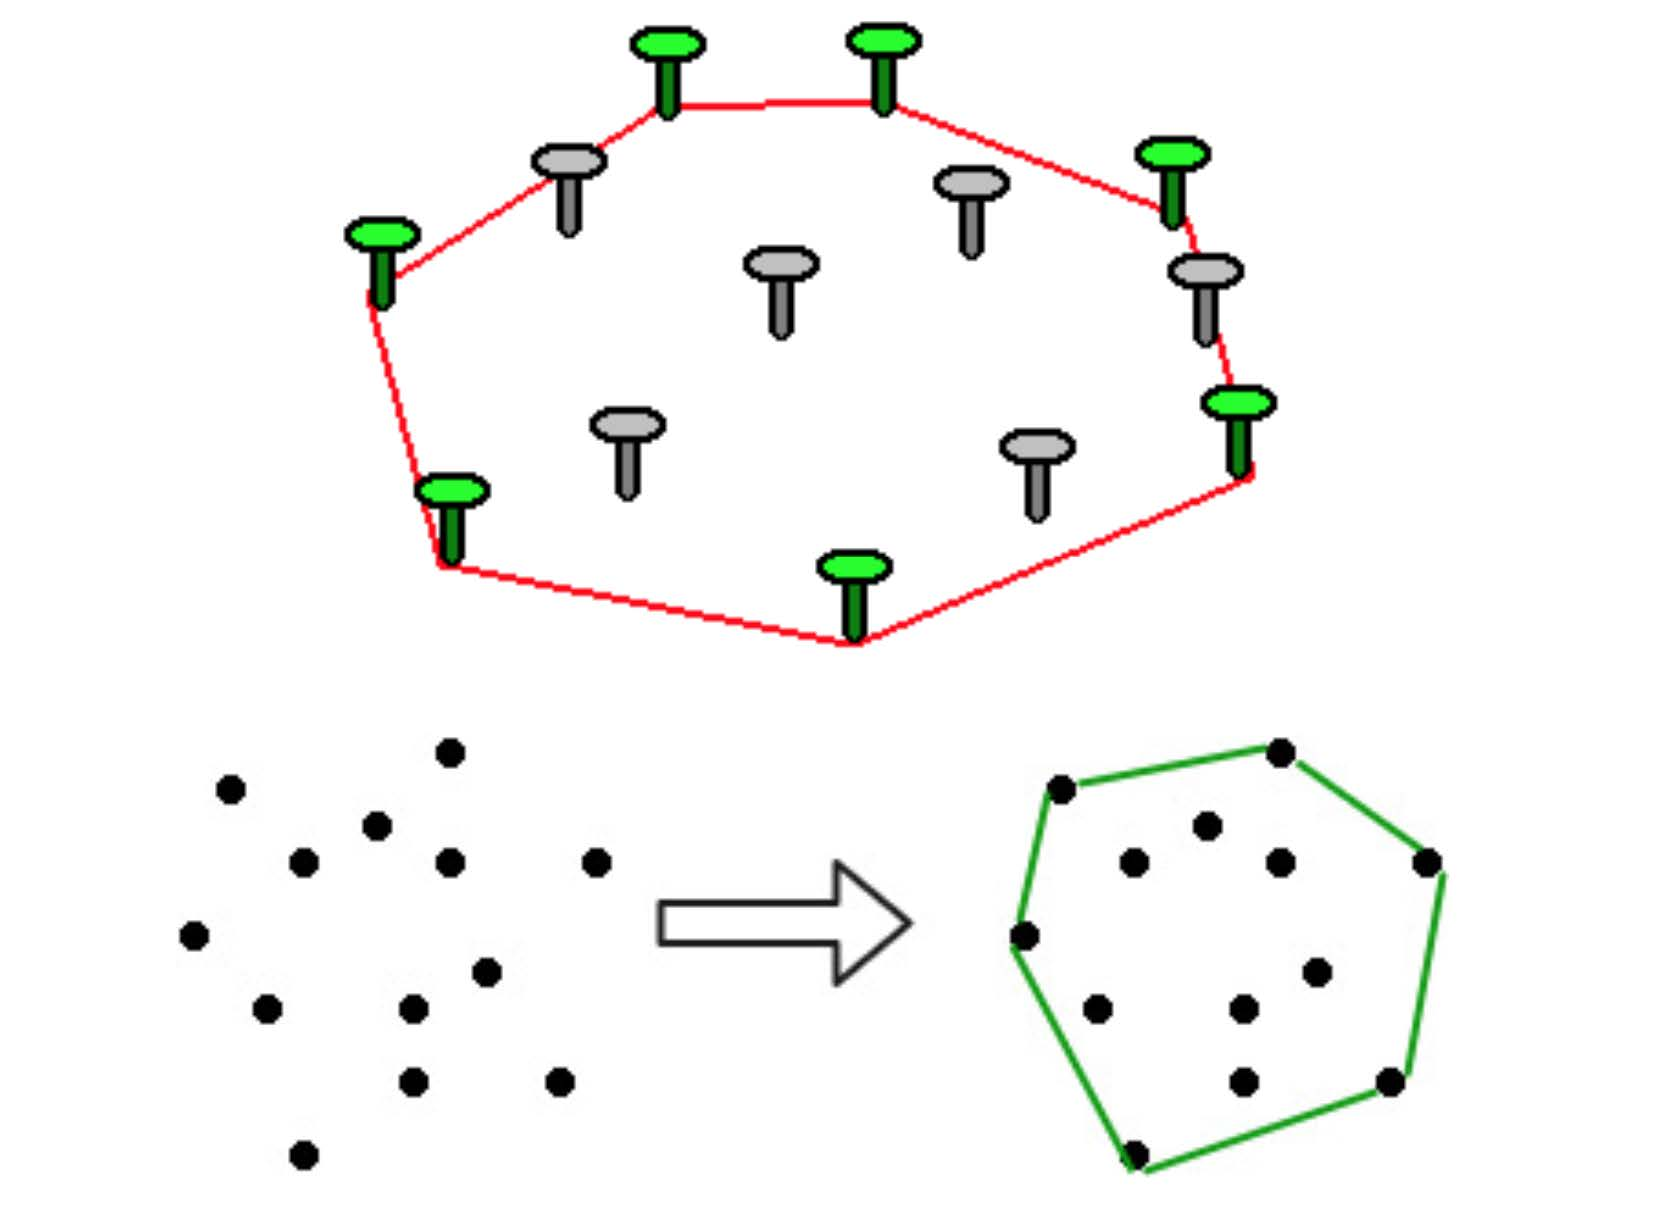
\includegraphics[width=\textwidth]{figs/L14-convex-hull.jpg}
        \end{figure}
    \end{columns}
\end{frame}


\begin{frame}{Jarvis algoritgm\cite{Jarvis1973}}

    Gift Wrap Algorithm (Jarvis March Algorithm) to find Convex Hull. 
    
    O(nh) complexity, where $n = \#S$, and h is the number of points on the
convex hull. Possition is checked by cross product.
        \begin{figure}
            \centering
            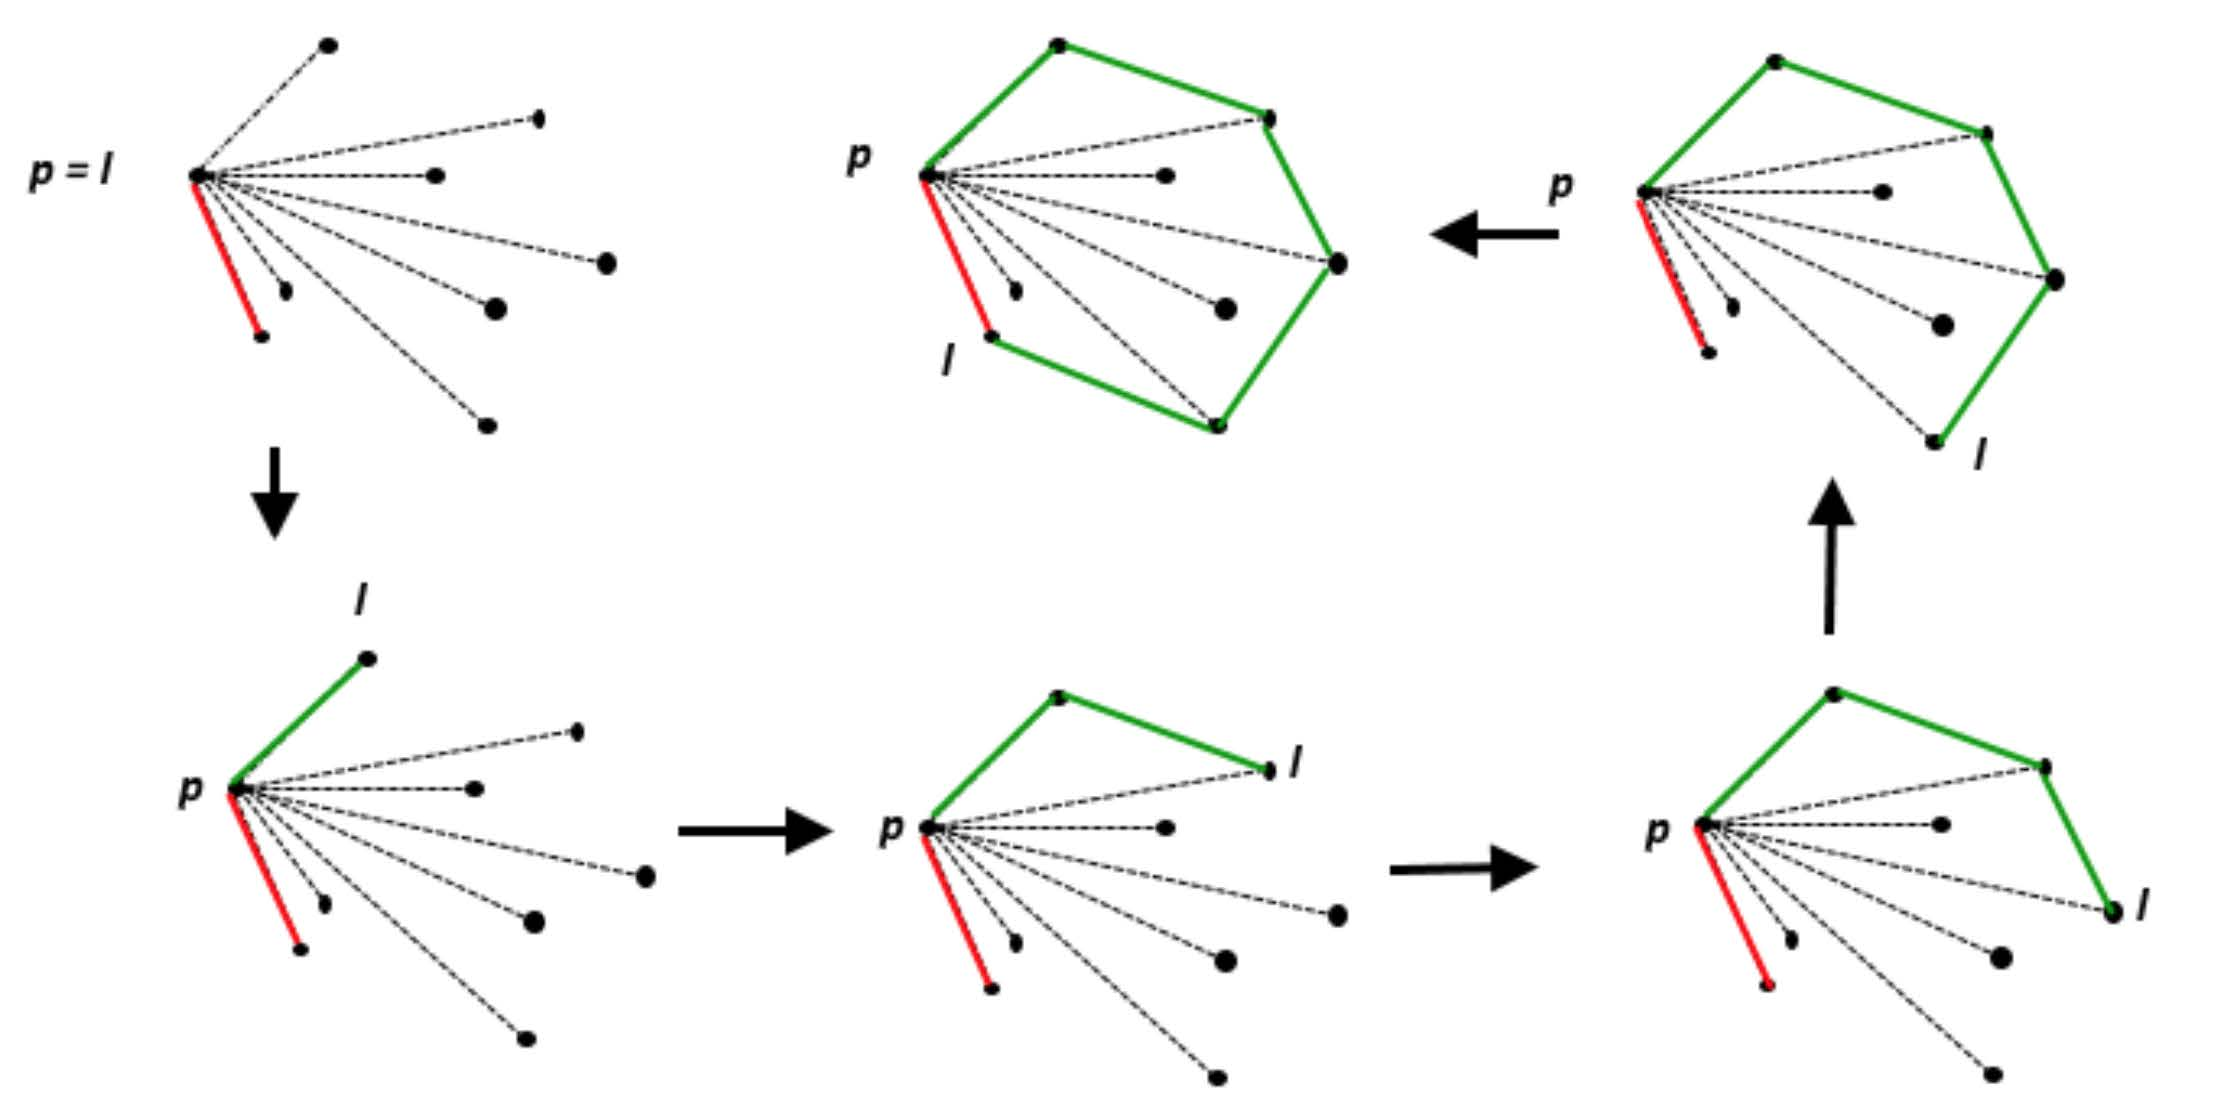
\includegraphics[width=\textwidth]{figs/L14-jarvis-algorithm.jpg}
        \end{figure}
    % \begin{columns}
    %     \column{0.7\textwidth}
    %     \column{0.3\textwidth}
    % \end{columns}
\end{frame}

\begin{frame}{Chan's algorithm\cite{Chan1996}}

Chan’s algorithm in the planar case: the algorithm combines an O(n log n)
algorithm (Graham scan-line, for example) with Jarvis march O(nh), in
order to obtain an optimal $O(n \mathrm{log} h)$ time.

    
\end{frame}

\begin{frame}{Alpha-complexes \cite{Edelsbrunner2010}}
    \begin{columns}
        \column{0.7\textwidth}
        \begin{figure}
            \centering
            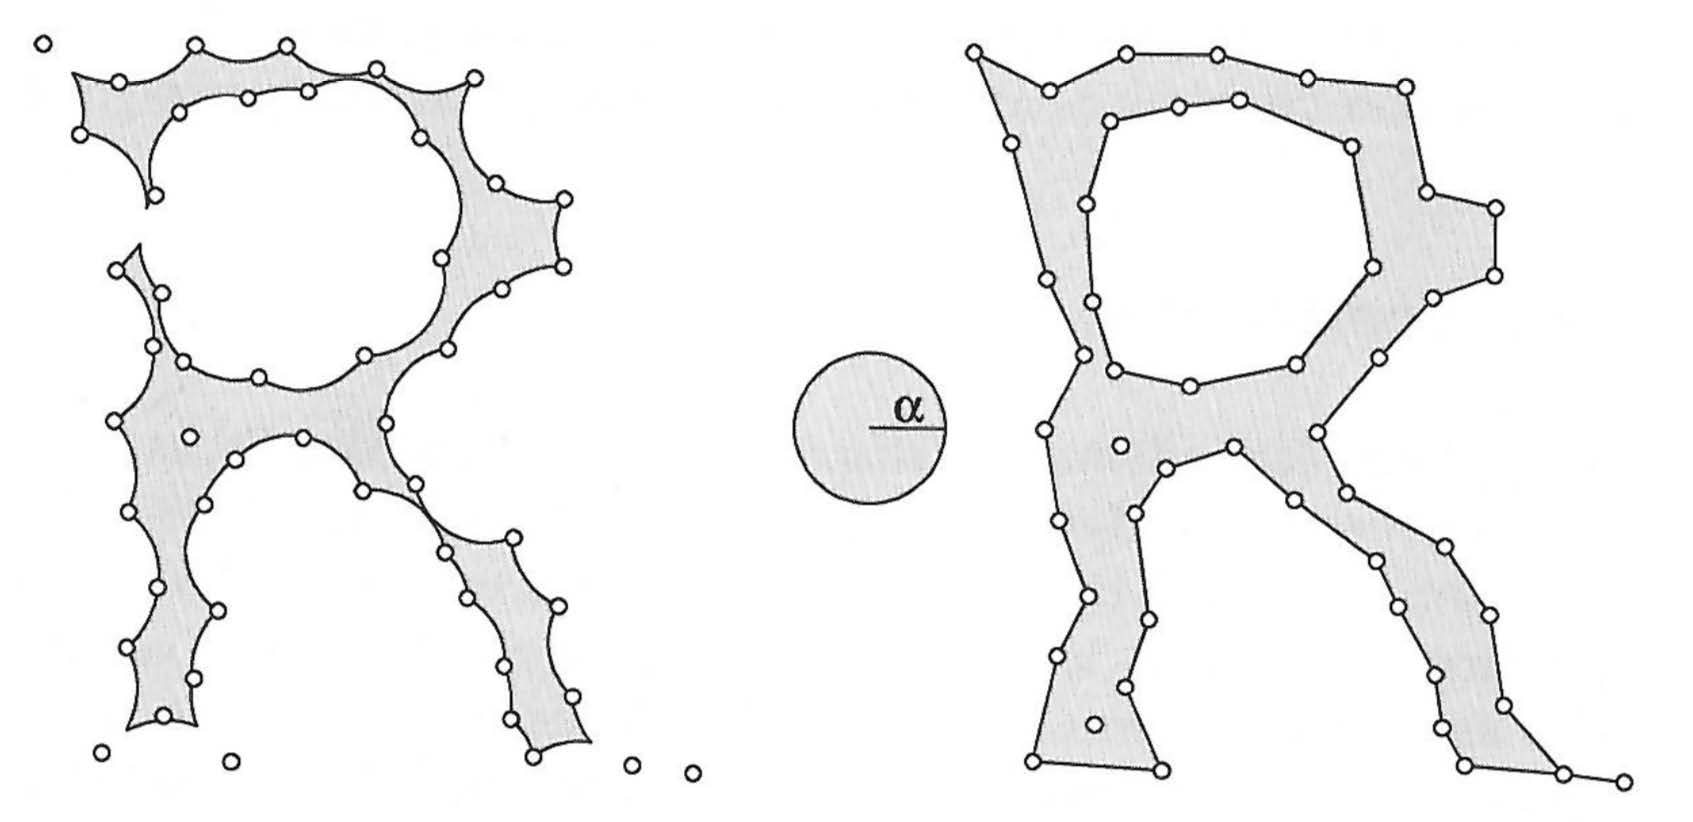
\includegraphics[width=\textwidth]{figs/L14-alpha-hull-alpha-shape.jpg}
            % \caption{Caption}
            % \label{fig:my_label}
        \end{figure}
        \column{0.3\textwidth}
        
    \end{columns}
\end{frame}

\begin{frame}{The Delaunay Triangulation}
    \begin{columns}
        \column{0.7\textwidth}
        \column{0.3\textwidth}
        \begin{figure}
            \centering
            % \includegraphics[width=\textwidth]{}
        \end{figure}
    \end{columns}
\end{frame}

\begin{frame}{Frame Title}
   	Herbert Edelsbrunner and John Harer, [Computational Topology. An Introduction](https://www.amazon.it/Computational-Topology-Introduction-Herbert-Edelsbrunner/dp/0821849255/),  AMS, 2011.

3.	Jeremy Kepner and John Gilbert,[Graph Algorithms in the Language of Linear Algebra](epubs.siam.org/doi/book/10.1137/1.9780898719918), 2011.

4.	Timothy A. Davis, [Direct Methods for Sparse Linear Systems](http://epubs.siam.org/doi/book/10.1137/1.9780898718881), SIAM, 2006

5.	Herbert Edelsbrunner, [Geometry and Topology for Mesh Generation](https://www.amazon.com/Generation-Cambridge-Monographs-Computational-Mathematics/dp/052168207X), Cambridge Monographs on Applied and Computational Mathematics, 2001. \cite{Edelsbrunner2001}
\end{frame}


\begin{frame}
	\frametitle{Content}
	\begin{itemize}
		\item Plain GAN
			\begin{itemize}
				\item[--] General Knowledge
				\item[--] Adversarial Loss
				\item[--] Problems of the training
				\item[--] Examples of Usage 
			\end{itemize}
		\item Autoencoders
			\begin{itemize}
				\item[--] Structure
				\item[--] Latent-space arithmetic
				\item[--] Variational Autoencoder
				\item[--] Examples of Usage 
			\end{itemize}
		\item Condi-GAN
			\begin{itemize}
				\item[--] General Knowledge
				\item[--] Examples of Usage 
			\end{itemize}
		
	\end{itemize}
\end{frame}

\endgroup

\begin{frame}{Interval Tree}

    
\end{frame}

\begin{frame}{Delaunay triangulations}

\cite{DeBerg2008}
    
\end{frame}